\section{Data}

%\subsection{Construction of Matrix $M$}
We seek to find values of $\alpha$ and $\beta$ that minimize the distance between rankings given by the bi-partite network random walker model, which takes the matrix $M$ as unique input, and ground-truth metrics on editor expertise and article quality, obtained independently from Wikipedia. We perform the model calibration for 13 snapshots (see Figure \ref{fig:snapshots})  for each of  the 12 categories of Wikipedia articles presented in Table \nolinebreak \ref{tab:statistics}. For each category and snapshot, we build the binary matrix $M$ by parsing all edit histories of all articles up to the snapshot time. We set $M_{ea} = 1$ for editor $e$ having modified article $a$, and $M_{ea} = 0$ otherwise. In order to eliminate page vandals, we considered only editors who made 5 or more edits to any article in the category. We also discarded all software robots (i.e. {\it bots}) that programmatically edit Wikipedia. 

\begin{table}
\begin{tabular}{|l|c|c|c|}
%\toprule
\hline
{\bf Category} &  {\bf Articles} &  {\bf Editors} &  {\bf Edits} \\
%\midrule
\hline
American male novelists               &      2,460 &   9,946 &  224,783 \\
2013 films                            &      1,896 &   5,215 &  150,956 \\
American women novelists              &      1,936 &   5,968 &  138,716 \\
Nobel Peace Prize laureates           &       104 &   4,165 &   91,522 \\
Sexual acts                           &        93 &   2,190 &   45,901 \\
Economic theories                     &       212 &   1,145 &   28,658 \\
Feminist writers                      &       233 &   1,357 &   25,738 \\
Yoga                                  &       123 &    730 &   25,315 \\
Military history of the US &       180 &    854 &   20,172 \\
Counterculture festivals              &        66 &    578 &   10,515 \\
Computability theory                  &        92 &    272 &    7,117 \\
Bicycle parts                         &        70 &    210 &    4,981 \\
\hline
\end{tabular}
\caption{Size statistics of investigated Wikipedia categories sorted by total edits.}
\label{tab:statistics}
\end{table}

\begin{figure}[!t]
\centering
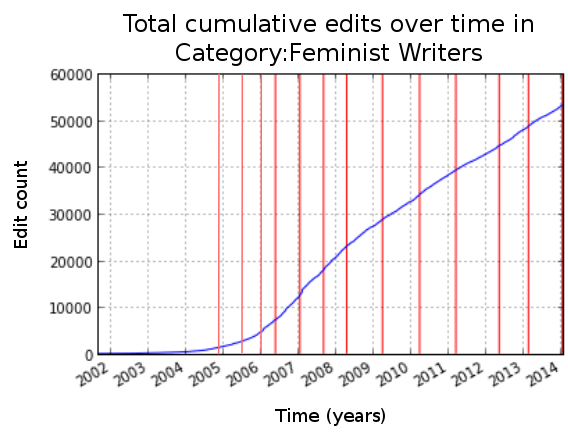
\includegraphics[width=0.9\columnwidth]{../Figures/cumulative_snapshots_Feminist_Writers_thirteen.png}
\caption{Cumulative edits made in Category {\it Feminist writers} (blue line). Vertical red lines represent the 13 snapshots taken at 2.5\%, 5\%, 7.5\% and then, 10\%, 20\%, 30\%, \ldots , 100\% of edits.}
\label{fig:snapshots}
\end{figure}

%\subsection{Editors Expertise and Articles Quality}
To calibrate $\alpha$ and $\beta$, we resorted to state-of-the-art ground-truth evaluations for editor expertise $\bar{w}_e$ and article quality $\bar{w}_a$. From these exogenous evaluations, we ranked editors and articles according to their expertise and quality respectively. We then performed  a grid search for values of $\alpha^*$ and $\beta^*$, which maximize the Spearman rank-correlation $\rho_e$ and $\rho_a$ between rankings obtained from the bi-partite random walker model $(w_e,w_a)$ and from exogenous metrics $(\bar{w}_e,\bar{w}_a)$. Actually, $(\alpha^*,\beta^*)$ must maximize both $\rho_e$ and $\rho_a$, even though $\rho_e$ and $\rho_a$ might actually be different. The optimization function  of $(\alpha^*,\beta^*)$ is given by,

\newcommand{\argmax}{\arg\!\max}

\begin{equation}
\begin{cases}
(\alpha^*,\beta^*) = \argmax_{\alpha, \beta}(\rho_e)\\
(\alpha^*,\beta^*) =\argmax_{\alpha, \beta}(\rho_a).\\
\end{cases}
\end{equation}

The set $(\alpha^*,\beta^*)$ characterizes how value flows from editors to articles, and from articles to editors, in the bi-partite network of collaboration in Wikipedia.

The ground-truth metrics were chose after a survey of the computer supported collaborative work literature. In the realm of quantifying editor qualit, there is a stream on editor "trust" from \cite{adler07} \cite{adler08} \cite{zeng}, parse the revision history to look at text survival rates. However we decided on \cite{geiger2013} and use "labor hours" for its refined yet simple technique which is inline with the rest of our parsimonous techniques. Labour hours accounts for the well decried fact that all edits are not equal, and rather counts the temporal length and editor has spend editing. It is calculated for each editor by taking contribution history up to the snapshot point. All edits made within 1 hour of a previous edit are counted in an {\it edit session}. If more than one hour separates two edits, a new period of edits  starts. The expertise expressed in labor hours is the sum of edit sessions. For the calculation of ground-truth expertise, we only consider edits for a given category, although the same editor might have edited other categories of articles in Wikipedia. 

In the case of article quality there are again many possible techniques from a collection of word-count related metrics \cite{blumenstock} to analyzing the momentum of the "diff" sequence \cite{wohner}. We selected metrics already in operation on Wikipedia \cite{wang2013tell} \cite{klein}, and have also been used in the CSCW literature in different combinations \cite{kane2011} \cite{keegan2012}. Our measure of actual article quality is performed through a combination of 5 text analysis metrics: (i) ratio of mark-up to readable text, (ii) number of headings, (iii) article length, (iv) citations per article length, (v) outgoing intra-Wiki links. We performed principal component analysis (PCA) for each category and snapshot in order to reduce dimensionality from 5 metrics to a single one (i.e. the principal component). The variance explained by the principal component varied between 0.5 and 0.72, confirming the dominance of the axis of maximum variance.

Since we are attempting to optimize the rank correlation between our model and ground-truth we must make the point on how they qualitatively differ, otherwise high correlations would come as no surprise. First lets turn our attention to editor rankings. Labor hours are focused around user editing and are completely agnostic to the page which has been edited. A single minded user spending 100 hours on a single article trying to get it to "Feature Article status" has made the same labor hour efforts as a user making 100 stub articles for an hour each. Yet depending on our amount of preferential attachment in our network, one or the other could be seen as a superior editor. Likewise on pages, an article text can be changed in 5 ways. The same edits could be made by one generalist editor or 5 specialist editors, and the ground-truth would not change. Depending on a different preferential attachment parameter in the model could rank each of these very differently.

Finally a point should be made about whether our exogenous expertise and quality measures are independent. Earlier on links between expert editors and quality articles were claimed \cite{wilkshuber}, and would seem intuitive. Yet, subsequently, there have been claims against such universal links which point out that key social interactions are not accounted for with these measures \cite{kane2009}. Intuitively this link rests on the collaborativeness of the articles and editors in question. With collaboration expertise will transtlate into article quality. However, given antagonistic, warring- editors expertise will not improve article quality.

